\documentclass[11pt, oneside]{article} 
\usepackage{geometry}
\geometry{letterpaper} 
\usepackage{graphicx}
	
\usepackage{amssymb}
\usepackage{amsmath}
\usepackage{parskip}
\usepackage{color}
\usepackage{hyperref}

\graphicspath{{/Users/telliott_admin/Tex/png/}}
% \begin{center} 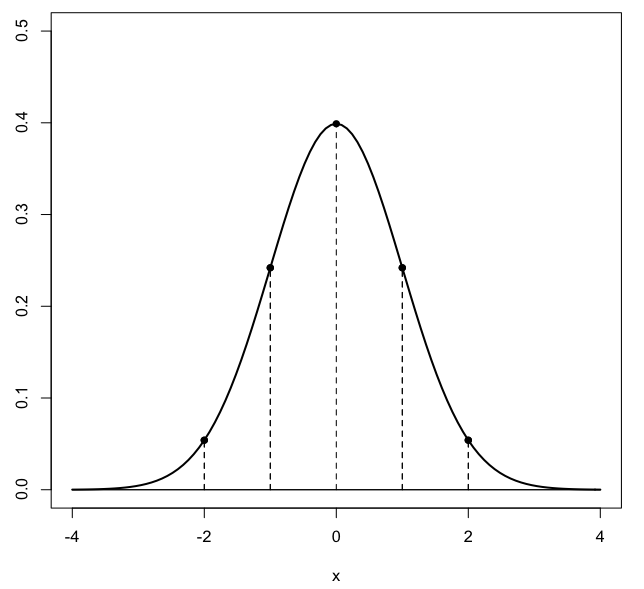
\includegraphics [scale=0.4] {gauss3.png} \end{center}

\title{Attraction of the earth}
\date{}

\begin{document}
\maketitle
\Large

\begin{center} 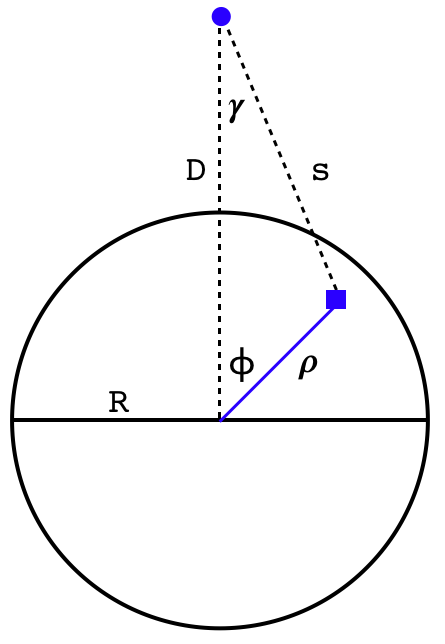
\includegraphics [scale=0.35] {newton_volume.png} \end{center}

We attack the same problem as we did in the previous chapter, except we set up the integral in a different way, one that allows us to solve a variant problem, that of the hollow sphere.

\subsection*{integral using $s$}
We repeat the analysis with $s$ as the variable.  Go back to the integral
\[ I = \int  \ [ \frac{1}{s^2} \cos \gamma \ ] \ \rho^2 \sin \phi \ d \phi  \]
\[ = \int \frac{1}{s^2} \ [ \  \frac{D^2 + s^2 - \rho^2}{2Ds}  \ ] \ \rho^2 \sin \phi \ d \phi \]
We need to get rid of $\sin \phi \ d \phi$, and turn it into something times $ds$.

The law of cosines for $\phi$ again:
\[ s^2 = D^2 + \rho^2 - 2 D \rho \cos \phi \]
Carry out implicit differentiation!  ($D$ and $\rho$ are constant).
\[ 2 s \ ds = 2 D \rho \sin \phi \ d \phi \]
\[ \frac{s}{D} \ ds =  \rho \sin \phi \ d \phi \]

So
\[ I = \int \frac{1}{s^2} \ [ \  \frac{D^2 + s^2 - \rho^2}{2Ds}  \ ] \ \rho \ \frac{s}{D} \ ds \]
\[ = \frac{\rho}{2D^2} \int \frac{1}{s^2} \ [ \  D^2 + s^2 - \rho^2  \ ] \ ds \]
Forget the leading factor for a moment, the integral is
\[ \int \ ds + \int \frac{D^2 - \rho^2}{s^2} \ ds \]
\[ = s - \frac{D^2 - \rho^2}{s} \]
\[ = s - \frac{(D + \rho)(D - \rho)}{s} \]
This might look somewhat familiar.

Now the question is, what are the bounds on $s$?  The minimum value is when $D$ is aligned with $\rho$ and $s = D - \rho$, while the maximum is the other way with $s = D + \rho$.  It is important that even though we have substituted $s$ for $\phi$ as the variable of integration, we are still doing this first integral with $\rho$ constant.

We must evaluate:
\[ s - \frac{(D + \rho)(D - \rho)}{s} \ \bigg |_{D - \rho}^{D + \rho} \]
This is exactly the same evaluation that we performed for the first integral!  The answer has not changed.

So what's the point?  

The thing is that now, we can move the test mass $m$ inside a hollow sphere easily.  To see how to do that, we set up the problem as a hollow sphere or shell problem.  However, the integral will be the one we just solved.

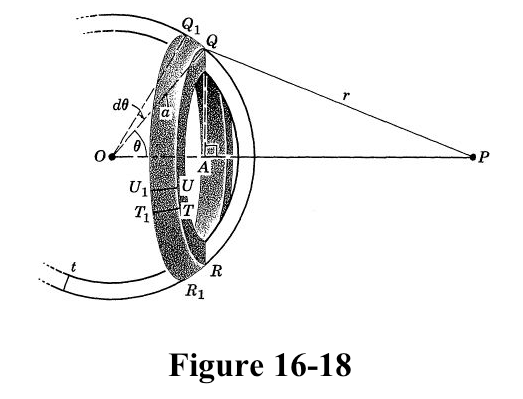
\includegraphics [scale=0.45] {Kline_16_18.png}  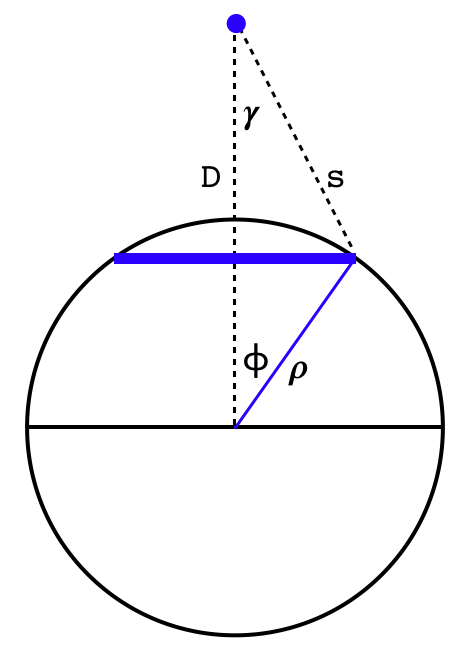
\includegraphics [scale=0.3] {newton_volume2.png}

We consider a band or belt of the hollow shell, where each piece is at a constant distance from the centerline.  In our notation the radius of the belt (a perpendicular dropped from the point $Q$ to point $A$ in the left-hand panel) is $\rho \sin \phi$.

The circumference of the belt is $2 \pi \rho \sin \phi$, the width is $\rho \ d \phi$ and so the surface area is
\[ A = 2 \pi \rho \sin \phi \ \rho \ d \phi \]
(The nice thing here is that $\rho d \phi$ gives the correct width of the belt easily.  We saw this approach before in looking at the moment of inertia for a sphere.

Following Kline, rather than calculate the mass, we take $t$ as the thickness of the (very thin) belt and $\mu$ as the density.  (This difference is not important to the argument).

$dM = \mu \ dV$ so the mass of the belt is
\[ dM = \mu t \ 2 \pi \rho^2 \sin \phi \ d \phi \]
and the total force on the test mass is
\[  \frac{Gm \mu t}{s^2} \ 2 \pi \rho^2 \sin \phi \ d \phi \]
The last part of the initial setup is that the net force is the component which acts along the central axis.  $dF$ is really
\[ dF = \frac{Gm \mu t}{s^2} \ 2 \pi \rho^2 \sin \phi \ d \phi \cdot \cos \gamma \]

If we were following the wikipedia derivation we would now get everything in terms of $\phi$ and integrate over $\phi = [0, \pi]$, but as we said above, Kline does something different.  He expresses all variables in terms of $s$ instead.
\begin{center} 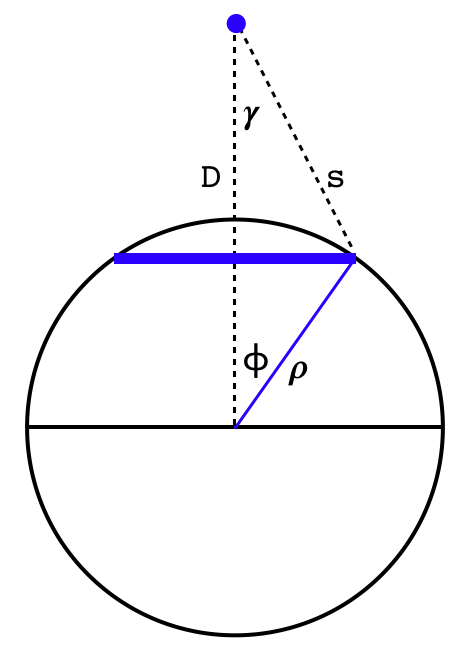
\includegraphics [scale=0.3] {newton_volume2.png} \end{center}
Rather than go through the law of cosines (we would get the same result), we can pretty much just read off the diagram, in the right triangle the side adjacent to $\phi$ is $\rho \cos \phi$, so the rest of $D$ is the side adjacent to $\gamma$, namely $D - \rho \cos \phi$ and
\[ \cos \gamma = \frac{D - \rho \cos \phi}{s} \]

This helps, but it's not all that we need.  We've exchanged $\gamma$ for $\phi$ and $s$, but we need all $s$ with no $\phi$.  From the law of cosines (yet again):
\[ s^2 = D^2 + \rho^2 - 2D \rho \cos \phi \]
Kline does a bit of clever algebraic manipulation.  Rearrange:
\[ s^2 - D^2 - \rho^2 = - 2D \rho \cos \phi \]
Add $2D^2$ to both sides
\[ s^2 + D^2 - \rho^2 = 2D^2 - 2D \rho \cos \phi \]
\[ \frac{s^2 + D^2 - \rho^2}{2D} = D - \rho \cos \phi \]
and thus
\[ \cos \gamma = \frac{D - \rho \cos \phi}{s}  =  \frac{s^2 + D^2 - \rho^2}{2Ds} \]
That takes care of $\gamma$.

Now rewrite the force as
\[ dF = \frac{Gm\mu t}{s^2} \ 2 \pi \rho^2 \ [ \ \frac{s^2 + D^2 - \rho^2}{2Ds} \ ] \ \sin \phi \ d \phi  \]

We still have $\sin \phi \ d \phi$.  We use this again:
\[ s^2 = D^2 + \rho^2 - 2D \rho \cos \phi \]
Carry out implicit differentiation as before:
\[ 2 s \ ds = - 2D \rho \ \sin \phi \ d \phi \]
\[ \sin \phi \ d \phi = \frac{s}{D \rho} \ ds \]
Back to the force
\[ dF = \frac{Gm \mu t}{s^2} \ 2 \pi \rho^2 \ [ \ \frac{s^2 + D^2 - \rho^2}{2Ds} \ ] \ \frac{s}{D \rho} \ ds \]

We are done with the fancy algebra.  Just cancel $2$, $s$ and $\rho$ top and bottom
\[ = \frac{Gm \mu t}{s^2} \ \pi \rho \ [ \ \frac{s^2 + D^2 - \rho^2}{D} \ ] \ \frac{1}{D} \ ds \]
Rearrange slightly
\[ = \frac{Gm \mu t \ \pi \rho}{D^2} \ [ \ \frac{s^2 + D^2 - \rho^2}{s^2} \ ] \ ds \]

This expression is what we have to integrate to get the total force.  Forget about the constant leading factor for a moment.  The integral is straightforward.  It breaks into two parts:
\[ \int \ [ \ 1 + \frac{D^2 - \rho^2}{s^2} \ ] \ ds \]
\[ = s - \frac{(D + \rho)(D - \rho)}{s} \]

And this is exactly the same one we already solved, with the same bounds.  The answer is $4 \rho$.  Picking up our leading factor, the force is
\[ F =  \frac{Gm \mu t \ 4 \pi \rho^2}{D^2} \]
Do you see that $4 \pi \rho^2 \ \mu t$ is the mass of the shell?  Call that mass $S$.  We have then
\[ F = \frac{GmS}{D^2}  \]
The mass $S$ acts in gravitation as if it were concentrated at the center, a distance $D$ from the test mass $m$.

To finish the problem, we need to add up an infinite number of infinitely thin shells ranging over the entire radius of the solid ball.  For this purpose, we return to
\[ F = \frac{Gm \mu t \ 4 \pi \rho^2}{D^2}  \]
Recall that $t$ is the thickness of a thin shell.  In the limit, this thickness is $d \rho$ so we have for the entire ball
\[ F = \int_0^R \frac{Gm \mu \ 4 \pi \rho^2}{D^2}  \ d \rho \]
but this is just
\[ = \frac{Gm \mu}{D^2} \ V  \]
and $\mu \ V$ is the entire mass of the ball so
\[ F = \frac{GmM}{D^2}  \]

This is exactly as we had before.  It is nice to do things by a different method and get the same answer.  However, we will now see another value of this approach.  As promised, the test mass moves inside the hollow sphere:

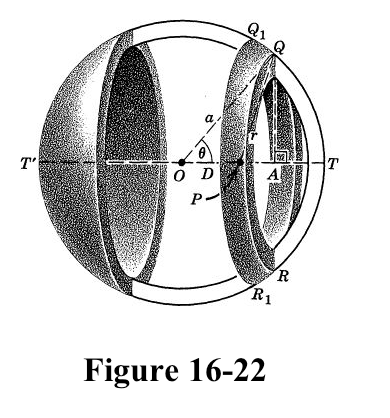
\includegraphics [scale=0.45] {Kline_16_22.png}  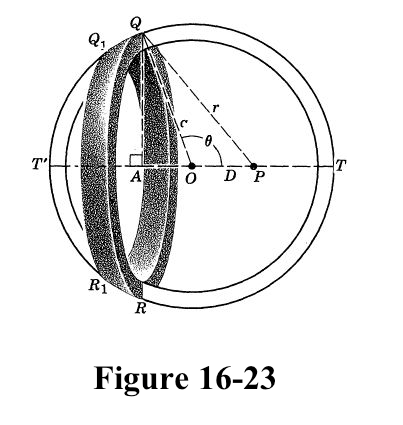
\includegraphics [scale=0.45] {Kline_16_23.png}

One change with the new setup is that $\phi$ may be obtuse when $P$ is inside.  That's OK, the law of cosines is still good even for an obtuse angle, which $\phi$ has become ($\theta$ in Kline's diagram Fig 16-23).

What is different and important is the \emph{bounds} on $s$.
\begin{center} 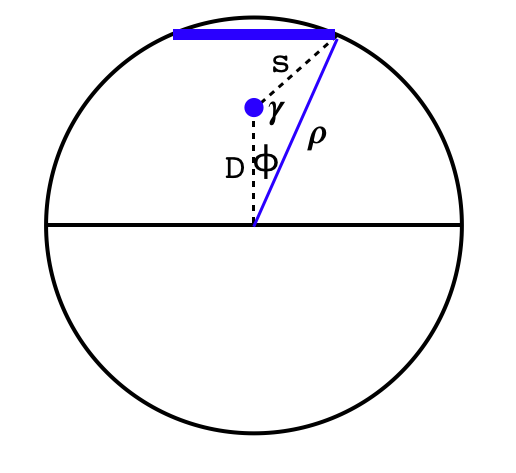
\includegraphics [scale=0.4] {newton_volume3.png} \end{center}

Now $D < \rho$ (the radius of the shell) and the bounds on $s$ have changed as well.

When $s$ extends to the very top on the same side of the shell where the point $P$ is located, $s + D = \rho$ so
\[s = \rho - D \]
while on the very bottom of the other side $s = \rho + D$.
\[ s = [\rho - D,\rho  + D] \]
This change of sign at the lower bound makes all the difference.

We evaluate the integral:
\[ s - \frac{(D + \rho)(D - \rho)}{s} \ \bigg |_{\rho - D}^{\rho + D} \]
At the upper bound, we get
\[ (\rho + D) - \frac{(D + \rho)(D - \rho)}{\rho + D} = 2 \rho \]
As before.  But at the lower bound
\[ (\rho - D) - \frac{(D + \rho)(D - \rho)}{\rho - D} \]
flip some signs
\[ = (\rho - D) + \frac{(D + \rho)(-D + \rho)}{\rho - D} \]
Canceling top and bottom
\[ (\rho - D) + (D + \rho) = 2 \rho \]

\emph{Subtracting} the latter from the former, we end up with zero.
There is no net force within the hollow sphere.

Now consider a solid ball, like the earth, and move inside as in the tunnel problem.

Imagine dividing the problem into two parts, break the ball into an outer hollow sphere, and an inner solid ball.  
\begin{center} 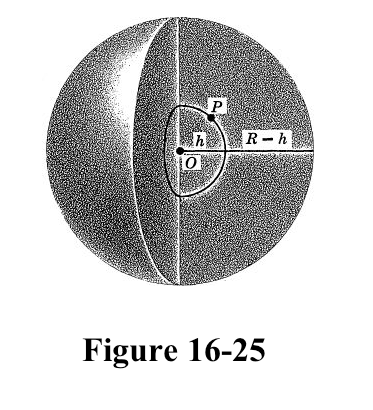
\includegraphics [scale=0.45] {Kline_16_25.png} \end{center}
The part outside the current location of the object exerts no net force.

The inner part exerts a force proportional to its mass, which is its relative volume times the total mass, over a distance which is smaller than initially.  If the distance penetrated is $h$, the effective mass is
\[  \frac{4/3 \pi h^3}{4/3 \pi R^3} M = \frac{h^3}{R^3} M \]
and the force is exerted over the new distance $h$ so we have
\[ F = Gm \  \frac{h^3}{R^3} M \ \frac{1}{h^2} = \frac{GmM}{R^2} \ \frac{h}{R} \]
as we said \hyperlink{Earth_tunnel}{\textbf{here}}.  A simple answer.


\end{document}